% !TEX root = ../thesis.tex
%\section{Inference on Markov Random Fields}

In this thesis, we consider the framework of Bayesian inference in Machine Learning where one is interested in combining prior knowledge about the parameters of a given model with the likelihood of the observed data given the model. 
This combination of prior and likelihood leads to a posterior distribution on the parameters which is the key object of interest in Bayesian inference. This can be written
\eqa{
	p(\theta\st\mathcal D) &\propto& p(\mathcal D\st  \theta) p(\theta)
} 
where $p(\theta)$ is the prior distribution function over the parameter of interest $\theta$, $p(\mathcal D\st \theta)$ denotes the likelihood of the data $\mathcal D$ for a given model parameter and $p(\theta\st \mathcal D)$ is the posterior distribution over the parameters. 

We focus on the problem of estimating expected values with respect to such a posterior distribution and in particular with respect to its marginals. 
Further, we consider the case where the posterior factorises in a specific way and consider methods that attempt to leverage the factorisation structure to offer estimators at a reduced computational cost. 
The thesis concentrates on computational methods to tackle the problem in a number of important cases as well as applications and experiments. 

The thesis is divided in two parts. In the first part -- \emph{Sampling Methods} -- we consider ``exact'' methods that attempt to produce samples from the true marginals and lead to estimators of expectations of interest that are exact in the limit of infinite computational power and infinite precision in the representation of numbers. These methods can work well when the dimensionality of the state-space associated with the marginals of interest is not too high. 

In the second part -- \emph{Approximate Bayesian Inference} -- we consider approximate methods that attempt to find proxies for the marginals in restricted probability distribution spaces. These methods can offer a viable alternative to sampling methods when the latter become too expensive to consider.\footnote{The separation between ``exact'' and ``approximate'' methods is a bit arbitrary. Another perspective can be to distinguish between ``sampling'' versus ``distributional'' approaches.}

In this introductory chapter we introduce the concept of Markov Random Fields and present a few classical examples.

%%%%%%%%%%%
\section{\label{subsection: mrf}Markov Random Fields}
A \margnote{MRF}\emph{Markov random field} (MRF) is a graph structure that represents joint distributions functions that factorise in a specific way or, in other words, to represent a set of conditional dependences between a set of random variables. In this document, we consider graphs determined by a finite index set $\mathcal V$, a set of edges $\mathcal E\subseteq \mathcal V\times \mathcal V$ connecting those nodes and \emph{potential functions} on its cliques (fully connected components of the graph). Each node $i\in\mathcal V$ corresponds to one random variable taking values in a sample space $\mathcal X_i \subseteq\mathbb R^{d_i}$ for some dimension $d_i\in\mathbb N$. 

We restrict ourselves to graphs with pairwise interactions i.e., uniquely determined by potential functions on their nodes and edges.\footnote{Considering only pairwise MRF is not too constraining since any MRF can be expressed as a pairwise MRF by the introduction of auxiliary variables although this may lead to a very complex graph \citep{yedidia00, wainwright08}.}
We write\check{sep14,jun22}
%
\eqa{	
	\psi_i : \mathcal X_i \to \mathbb R^{+}, \quad \text{and}\quad \psi_{ij}: \mathcal X_i\times \mathcal X_j \to \mathbb R^{+}, \nn	
}
% 
respectively a potential function on a node $i\in \mathcal V$ and on an edge $(i,j)\in \mathcal E$. 
%Note that, in principle, any MRF can be 
Such a graph represents the factorisation structure of a class of probability density functions on the product space $\mathcal X := \prod_{i\in \mathcal V}\mathcal X_{i}$ that can be written as
\eqa{		p(x) &\propto & \prod_{i\in\mathcal V}\psi_{i}(x_{i})\prod_{j\in\partial i}\psi_{ij}(x_{i},x_{j}),	}
where $x=(x_{i})_{i\in \mathcal V}$ and $\partial i:=\{j\st (i,j)\!\in\,\!\mathcal E\}$ denotes the \emph{neighbourhood} of the $i$th node. 
A simple pairwise MRF is illustrated in \fig{fig:simple-MRF}.\\

\begin{figure}[!h]
\center
\begin{tikzpicture}[-,>=stealth',shorten >=1pt,minimum size=0.8cm,scale=.1,node distance=1.5cm, thick]
	\node[circle,draw] (A) 						{$w$};
	\node[circle,draw] (B) [above of=A] 		{$x$};
	\node[circle,draw] (C) [below right of=A] 	{$z$};
	\node[circle,draw] (D) [below left of=A] 	{$y$};
	
	\path 
	(A) edge	(B)
	(A) edge	(C)
	(A) edge	(D)
	;
\end{tikzpicture}
\caption{\label{fig:simple-MRF}Illustration of a simple MRF corresponding to distributions over 4 random variables admitting the following factorisation structure:\\ $p(w,x,y,z)\propto \psi_{w}(w)\psi_{x}(x)\psi_{y}(y)\psi_{z}(z)\psi_{wx}(w,x)\psi_{wz}(w,z)\psi_{wy}(w,y)$.}
\end{figure}
%The node potentials usually correspond to the likelihood of some observations $y_i$ (possibly a collection of observations) such that they can be written
%\eqa{ \psi_i(x_i) &=& p_i(y_i\st x_i),	\nn	}
%for some likelihood model $p_i$.
In this work, we are mainly concerned in determining or approximating  \emph{marginals}\margnote{marginals} on the MRF i.e. the distributions $p_{\mathcal I}(x_{\mathcal I})$ for $\mathcal I\subseteq\mathcal V$  with
\eqa{		p_{\mathcal I}(x_{\mathcal I}) &:=& \int p(x)\dx_{\mathcal V\backslash\mathcal I},	\label{eq:marginals}}
where the integral is implicitly taken over $\prod_{i\notin I}\mathcal X_{i}$.\\
A particular case of interest is\, $\mathcal I=\{r\}$ corresponding to the case of singleton marginals \citep[section 2.3]{wainwright08}. The integrals of the form \eqref{eq:marginals} are typically intractable but exploiting the underlying factorisation structure can lead to good approximation methods.\check{sep14, sep14, jun22}

We distinguish between two classes of undirected graph structures: the connected acyclic ones (\emph{trees}) and the rest (\emph{loopy graphs}). As we will show, computing marginals on a tree is relatively simple in comparison to doing so on loopy graphs. 
Among the trees, two graph structures are of particular interest in this document: the \emph{chain graph} and the \emph{star graph}. 
We also illustrate one specific type of loopy graph: the \emph{grid graph}.

%\dred{COULD ADD hierarchical model as tree graph}

%%%%%%%%%%%
\section{\label{intro:exMRF}Examples of MRF}
In this section, we present a brief overview of three examples of graph structures on which we will focus most of our effort throughout this document. 
We also present the type of applications they are connected with. 

%%%%%%%%%%%%%%
\subsection{Hidden Markov Models}
Chain graphs, where the random variables on every node take value in the same state-space $\mathcal X$, form the underlying structure of \emph{Hidden Markov Models} (HMM)\margnote{HMM} an important class of models. These can be illustrated as follows:
\begin{figure}[!h]
\center
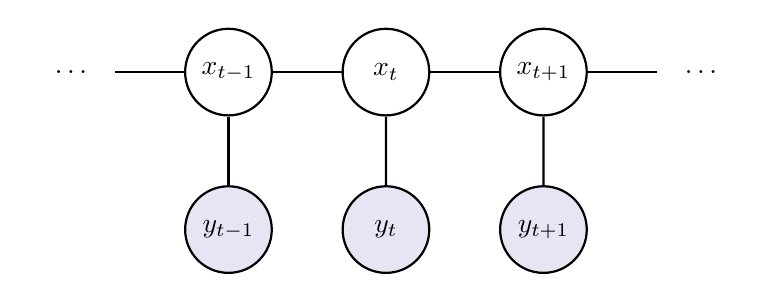
\begin{tikzpicture}[-,minimum size=1.1cm,scale=.1,node distance=2cm, thick]
	\node[circle,draw] (A) {$x_{t-1}$};
	\node[circle,draw] (B)[right of=A] {$x_{t}$};
	\node[circle,draw] (C) [right of=B] {$x_{t+1}$};
	\node[] (D) [right of=C] 	{$\dots$};
	\node[] (E) [left of=A]		{$\dots$};
	\node[circle,fill=DarkBlue!10,draw] (F) [below of=A] {$y_{t-1}$};
	\node[circle,fill=DarkBlue!10,draw] (G) [below of=B] {$y_{t}$};
	\node[circle,fill=DarkBlue!10,draw] (H) [below of=C] {$y_{t+1}$};
	
	\path 
	(A) edge	(B)
	(B) edge	(C)
	(C) edge	(D)
	(E) edge	(A)
	(A) edge (F)
	(B) edge (G)
	(C) edge (H)
	;
\end{tikzpicture}
\caption{\label{fig: hmm1} HMM with states $\{x_{t}\}_{t=1}^{T}$ and observations $\{y_{t}\}_{t=1}^{T}$.}
\end{figure}

HMMs are used in a broad range of applications from modelling time series data to speech processing (see for example \citet{ghahramani01, gales07, zucchini16}). In HMMs, the node potentials correspond to the likelihood of the corresponding observation and the edge potentials correspond to the \emph{transition density}:
\eqa{	\psi_t (x_t) &=& p(y_t\st x_t), \quad\text{and}\quad \psi_{t-1,t}(x_{t-1},x_t) \spe p(x_t\st x_{t-1}).	\nn}
A prior $\pi_{0}\in\mathcal P(\mathcal X)$ is assumed to be given for the first node so that we can write $p(x_1\st y_{1}) \propto \pi_{0}(x_1)p(y_1\st x_1)$. \check{sep14}

In the case of the HMM, obtaining or approximating the singleton marginals on the nodes from $1$ to $T$ given the observations $y_{1:T}$ is known as a \emph{smoothing problem}\margnote{smoothing}. The marginals or \emph{smoothing densities} can be written $p(x_t\st y_{1:T})$ to make explicit the dependence on all available observations.

A related problem is the \emph{filtering problem}\margnote{filtering} where one is only interested in building the last singleton marginal or, to put the problem in the same framework as before, to build marginals taking into account only the observations available until the point considered. This can be useful in an online setting where one is streaming data. 
The filtering densities are written $p(x_t\st y_{1:t})$. Correspondingly, we are often interested in representing the prediction density obtained by integrating the filtering densities with the transition density: 
%
\eqa{
	p(x_{t+1}\st y_{1:t}) &\propto& \int p(x_{t+1}\st x_{t}) p(x_{t}\st y_{1:t})\dx_{t}.
	}
%
%A related problem is to approximate the smoothing densities: $p(x_{t}\st y_{1:T}$). We will explore this in more details in chapter \ref{chap:BIS}. \check{jul24,june22}
%This is particularly relevant for applications such as time series analysis.\\

The \emph{linear-Gaussian} case is a particular instance of HMM, usually expressed as:
\eqa{	\syst{
			\pi_{0}(x_1) 				&=& \mathcal N(x_1; \mu_0, Q_0)	 	\\
			p(x_t\st x_{t-1}) 	&=& \mathcal N(x_t; A_t x_{t-1}+a_t, Q_t)		\\
			p(y_t\st x_t) 		&=& \mathcal N(y_t; B_t x_t+b_t, R_t)
		}
	\nn}
where $\mu_0$ as well as the $Q_t$, $R_t$, $A_t$, $a_t$, $B_t$ and the $b_t$ are fixed and deterministic. In such a case, an analytical expression for both the filtering and the smoothing densities can be obtained through the well-known \emph{Kalman filter} and \emph{Kalman smoother} \citep{anderson79}. \check{sep14}

However, in the general case where the transition is nonlinear and/or non-Gaussian, the marginals are typically intractable. Approximation algorithms such as \emph{Sequential Monte Carlo methods} (SMC) have been developed in order to generate approximate samples from these marginals and consequently be able to form Monte Carlo estimators. We introduce these methods in more detail in chapter \ref{chap:BGsampling}.
%We will show in this document a novel method to exploit a variational method known as \emph{expectation propagation} to help the performances of SMC smoothing algorithms. \dred{ADD SECTION NUMBER}

%%%%%%%%%%%%%%
\subsection{Star graphs}

In this document, we define \emph{star graphs}\margnote{star graph} as corresponding to a structure with a single random variable (possibly high-dimensional) with a node potential that factors into several likelihood terms. The structure is illustrated in figure \ref{fig:star1}. 

\begin{figure}[!h]
\center
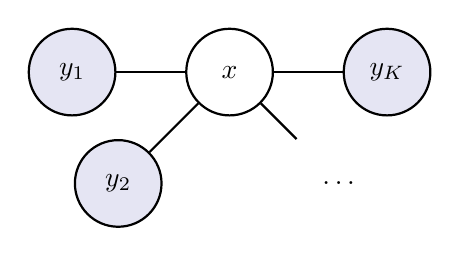
\begin{tikzpicture}[-,minimum size=1.1cm,scale=.1,node distance=2cm, thick]
	\node[circle,draw] (A) {$x$};
	\node[circle,fill=DarkBlue!10,draw] (B) [left of=A]		   {$y_{1}$};
	\node[circle,fill=DarkBlue!10,draw] (C) [below left of=A]  {$y_{2}$};
	\node[] (D) [below right of=A] {\dots};
	\node[circle,fill=DarkBlue!10,draw] (E) [right of=A]  {$y_{K}$};
	
	\path 
	(A) edge	(B)
	(A) edge	(C)
	(A) edge	(D)
	(A) edge (E)
	;
\end{tikzpicture}
\caption{\label{fig:star1} Star graph with hidden state $x$ and observations $\{y_k\}_{k=1}^{K}$. }
\end{figure} 

In this case, the singleton marginal can simply be written as:
\eqa{	p(x\st y) &\propto& \pi_0(x) \prod_{i=1}^{K} p(y_k\st x)	\nn}
where the $y_k$ are subsets of the entire observed data and $\pi_0$ is a prior on the hidden state. 
This can be a useful representation for distributed inference where each of the observation nodes can correspond to a distinct physical machine with a portion of the relevant data. 
We exploit this structure to suggest a novel way to approach distributed Bayesian inference in chapter \ref{chap:EPforDBI}.\check{sep14, jul24, jun21}

\subsection{Grid and loopy graphs}
The examples listed above do not exhibit cycles. An example of a common MRF structure with cycles which is encountered, for instance, in image processing, is the \emph{grid graph}\margnote{grid graph} illustrated in \fig{fig:grid1}.

\begin{figure}[!h]
	\center
	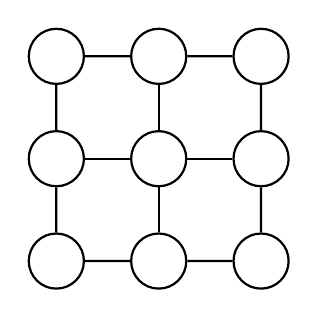
\begin{tikzpicture}[-,minimum size=.7cm,scale=.1,node distance=1.3cm, thick]
		\node[circle,draw] (A){};
		\node[circle,draw] (B) [left  of=A] {};
		\node[circle,draw] (C) [right of=A]{};
		\node[circle,draw] (D) [below of=A]{};
		\node[circle,draw] (E) [above of=A]{};
		\node[circle,draw] (F) [above of=B]{};
		\node[circle,draw] (G) [above of=C]{};
		\node[circle,draw] (H) [below of=B]{};
		\node[circle,draw] (I) [below of=C]{};
		\path
		(A) edge (B)
		(A) edge (C)
		(A) edge (D)
		(A) edge (E)
		(B) edge (F)
		(B) edge (H)
		(C) edge (I)
		(C) edge (G)
		(F) edge (E)
		(E) edge (G)
		(H) edge (D)
		(D) edge (I)
		;
	\end{tikzpicture}
\caption{\label{fig:grid1} Generic structure of a grid graph.}
\end{figure}

In image processing, grid graphs can be used to model interactions between the pixels of an image  \citep{blake11}. 
In the case of image denoising for example, for each pixel $k$ a noisy value $y_k$ is observed and we can have a model for the likelihood of $y_k$ given the true pixel value $x_k$ in the form $p(y_k\st x_k)$. These  form the node potentials. 
Additionally, we may have a similarity measure which can be used to penalise neighbouring pixels being very dissimilar. These form the edge potentials.\\
The problem of finding or approximating the singleton marginals then corresponds to finding the likelihood of a particular pixel taking a specific value given all the noisy observations available. We consider the problem of approximating marginals on such loopy graphs in chapter \ref{chap:EPBP}. \check{sep14, jul24,jun21}

\section{Exact vs Inexact Methods and Structure of the Thesis}

While the unifying theme of this thesis is the inference problem on Markov Random Fields, we consider two rather different approaches forming the two main parts of the thesis. In the first approach -- \emph{sampling methods} -- we consider methods to produce samples from the target densities (marginals of an MRF) from which Monte Carlo estimators can be computed. These methods take the form of stochastic processes which, asymptotically, are guaranteed to generate samples from the target distribution. These methods are considered ``exact'' because, asymptotically, they yield samples from the correct distribution. The difficulty of course is to assess whether the generating process has converged in the context of finite compute time and finite precision arithmetics. 

In the second approach -- \emph{approximated Bayesian inference} -- we consider methods to produce proxies to the target densities and compute expected values with respect to these proxies. These methods are considered ``inexact'' because even in the limit of infinite computational power or infinite precision arithmetic they do not lead to the correct expected values. 

Formally, let us denote $p$ a target distribution of interest and $\varphi$ a test function and put ourselves in the realistic context of finite computational power and precision. The aim is to compute the expected value of $\varphi$ with respect to $p$ or $\E_{p}[\varphi(X)]$. The first class of methods generates incorrect samples $\{\hat x_{1},\dots,\hat x_{n}\}$ which are hopefully statistically not too far from exact (but usually inaccessible) samples $\{x_{1},\dots,x_{n}\}$ drawn iid from $p$. 
As will be covered in section \ref{sec:MC+SMC}, the expected value of interest will be approximated as $\E_{p}[\varphi(X)]\approx n\inv \sum_{i=1:n}\varphi(\hat x_{i})$. The second class of methods attempts to find a simple distribution $q$ which is close in some sense to the target distribution $p$, the expected value of interest is consequently approximated as $\E_{p}[\varphi(X)]\approx \E_{q}[\varphi(X)]$. 

These two approaches rely on different sets of tools. 
The first one relies primarily on sampling/particle methods while the second relies more heavily on optimisation tools. 
To simplify the presentation of the thesis, we therefore have two background chapters beginning each of the two parts. Each part is then formed of two chapters covering a specific method and discussing applications. 


%The two approaches consider fairly different tools as 
%
%For both hard to assess qual... 



